\section{Das Objektsystem von Racket: Onstage}
Als Grundlage für dieses Kapitel dient die Racket-Dokumentation \cite{racketguide-classes} und -Referenz \cite{racketref-classes} für Klassen und Objekte.

Racket ist eine Multipurpose-Sprache und erlaubt die Auswahl der Syntax auf Sprachebene. Eine einzelne Codezeile bestimmt die Sprache eines Moduls, also beispielsweise, ob die Funktionen vorgezogen ausgewertet werden (\texttt{\#lang racket}) oder verzögert (\texttt{\#lang lazy}). Da das Objektsystem in die Sprache Racket integiert ist, kann man es direkt in jedem Racket-Modul verwenden.

% \begin{lstlisting}
%  #lang racket
% \end{lstlisting}

Die wichtigsten Werkzeuge, die man als Programmierer in einer objektorientierten Sprache benötigt, sind das Definieren von Klassen, Feldern und Funktionen, sowie das Erzeugen von Objekten. Auf diese soll deshalb im Folgenden kurz eingegangen werden, bevor wir dazu kommen, welche Möglichkeiten es in Bezug auf Mehrfachvererbung im Objektsystem von Racket bereits gibt.

Alle Code-Beispiele sind auch noch einmal zusammenhängend in Anhang \ref{or-example} aufgeführt. 

\subsection{Einfache Klassen}

Eine Klasse wird in Racket durch das Schlüsselwort \texttt{class} definiert. Bei der Definition einer Klasse muss die Superklasse angegeben werden. Falls die Klasse keine (anderen) Superklassen hat, wird \texttt{object\%} angegeben, die eingebaute Wurzelklasse. Per Konvention sollen Klassennamen in Racket auf \% ended, bei den folgenden Beispielen wird jedoch darauf verzichtet, um sie später leichter mit CLOS vergleichen zu können. Nach der Superklasse können noch beliebige Klassenoptionen, Felder oder Methoden definiert werden. An einer beliebigen Stelle im Rumpf der Klasse muss jedoch mit \texttt{super-new} der Konstruktor der Oberklasse aufgerufen werden. Eine minimale Klassendefinition sieht damit folgendermaßen aus:

\begin{lstlisting}
(class object% (super-new))
\end{lstlisting}

Als Rückgabewert erhält man ein Klassenobjekt und kann dieses für den späteren Zugriff in einer Variablen speichern. Die Variable wurde hier Thing genannt.

\begin{lstlisting}
(define Thing (class object% (super-new)))
\end{lstlisting}

Objekte von Klassen lassen sich mit dem Schlüsselwort \texttt{new} erzeugen:

\begin{lstlisting}
(new Thing)
\end{lstlisting}

Felder lassen sich mit \texttt{init-field} oder \texttt{field} deklarieren, je nachdem, ob es möglich sein soll sie bei der Objekterzeugung zu initialisieren oder nicht. Auf die Felder kann man dann mit \texttt{get-field} beziehungsweise \texttt{set-field!} zugreifen. 

Für Methoden gibt es, je nach Art und Sichtbarkeit, unter anderem die Schlüsselwörter \texttt{define/public}, \texttt{define/private} und \texttt{define/override}. Die so definierten Methoden lassen sich anschließend mittels \texttt{send} aufrufen. Zum Beispiel sieht eine Klasse namens Element, bestehend aus einem Feld für das Attribut und einer sondierenden Methode, die von Thing erbt, folgendermaßen aus:

\begin{lstlisting}
(define Element (class Thing (super-new)
                  (init-field [attr 'water])
                  (define/public (hot?) (equal? attr 'fire))))
\end{lstlisting}

Attribute, die keinen Defaultwert haben, müssen bei der Initialisierung angegeben werden. Da das Attribut der Element-Klasse, hier \texttt{attr} genannt, \texttt{{\textquotesingle}water} als Defaultwert hat, ist eine Angabe bei der Objekterzeugung optional. Mit den Methoden \texttt{get-attr} und \texttt{set-attr} können wir darauf zugreifen:

% > elem
% \end{lstlisting} 
% {\routput (object:Element ...)}

\begin{lstlisting}
(define elem (new Element))

> (get-field attr elem)
\end{lstlisting} 
{\rsymbol{water}}
\begin{lstlisting}
> (send elem hot?)
\end{lstlisting} 
{\routput{\#f}}

\begin{lstlisting}
> (set-field! elem attr 'fire)
> (send elem hot?)
\end{lstlisting} 
{\routput{\#t}}
% 
% \begin{lstlisting}
% (define elem2 (new Element [attr 'fire]))
% 
% > (send elem2 get-attr)
% \end{lstlisting} 
% {\rsymbol{fire}}

Wir können uns auch eine Klasse Animal definieren, die von Thing erbt (auch wenn es nicht viel zu vererben gibt):

\begin{lstlisting}
(define Animal (class Thing (super-new)
                 (init-field [gender 'male]
                             [size 'small])))
\end{lstlisting} 

Und eine Klasse Pet, die wiederum von Animal erbt:

\begin{lstlisting}
(define Pet (class Animal (super-new)
              (init-field [name 'unknown])))
\end{lstlisting} 

Objekte der Klasse Pet besitzen dann alle drei Attribute:

\begin{lstlisting}
(define harry (new Pet [name 'harry] [size 'normal]))

> (get-field name harry)
\end{lstlisting} 
{\rsymbol harry}

\begin{lstlisting}
> (get-field gender harry)
\end{lstlisting} 
{\rsymbol male}

\begin{lstlisting}
> (get-field size harry)
\end{lstlisting} 
{\rsymbol normal}

% TODO The make-object procedure creates a new object with by-position initialization arguments, the new form creates a new object with by-name initialization arguments, and the instantiate form creates a new object with both by-position and by-name initialization arguments.

\subsection{Mehrfachvererbung in Racket}
Zuvor wurde behauptet, mit Racket könne man keine Mehrfachvererbung modellieren. Tatsächlich gibt es zwei Arten von Klassen in Racket, deren Verhalten auf den ersten Blick wie Mehrfachvererbung aussieht: Mixins und Traits. Es werden deshalb beide kurz vorgestellt, um aufzuzeigen, welche Probleme und Grenzen sie haben.

Dafür verwenden wir unsere vorher definierten Klassen Element und Animal. Beide haben unterschiedliche Felder und Methoden. Wir wollen versuchen, die Felder und Methoden aus beiden in einer neuen Klasse namens Pokemon zu vereinigen (Abbildung \ref{hirarchy}). Das ginge natürlich ganz simpel, indem eine der beiden Klassen in Pokemon umbenannt wird und von der anderen erbt, deshalb wollen wir außerdem fordern, dass beide Klassen auch einzeln verwendet können. 

\begin{figure}[h]
 \centering
 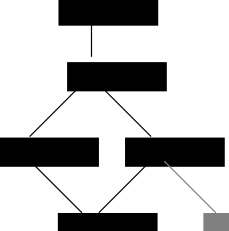
\includegraphics[width=0.35\textwidth]{pictures/hirarchy}
 \caption{Vererbungshierarchie für die Klasse Pokemon.}
 \label{hirarchy}
\end{figure}


\subsubsection{Mixins}
Die Auswertung eines \texttt{class}-Aufrufs gibt uns ein Klassenobjekt zurück. Es möglich, dieses als Parameter an Funktionen oder andere Klassen zu übergeben oder auch als Rückgabewert eines Funktionsaufruf zu definieren. Wir könnten uns beispielsweise eine Methode \texttt{generate-subclass} definieren, die eine Klasse als Parameter erhält und eine Subklasse von dieser erzeugt. Dafür muss sie den Parameter nur als Superklasse in einer Klassendefinition verwenden:

\begin{lstlisting}
(define (generate-subclass superclass)
  (class superclass (super-new)))
\end{lstlisting} 

Das ist noch keine sonderlich spannende Subklasse, da sie sich genauso verhält wie die angegebene Superklasse.
% aber wir können uns von ihrer Funktionalität überzeugen. Nehmen wir beispielsweise eine Subklasse der Klasse Element:
% 
% \begin{lstlisting}
% > (generate-subclass Element) 
% \end{lstlisting}
% {\routput \#<class:...>}
% 
% Dann erhalten wir das gleiche Verhalten wie für Objekte der Klasse Element:
% 
% \begin{lstlisting}
% > (new (generate-subclass Element))
% \end{lstlisting}
% {\routput (object:...)}
% 
% \begin{lstlisting}
% > (send (new (generate-subclass Element)) get-attr)
% \end{lstlisting}
% {\rsymbol water}
% 
Nun könnte man in der in \texttt{generate-} \texttt{subclass} definierten Klasse natürlich auch noch weitere Felder und Methoden hinzufügen. Die Klasse fügt dann Verhalten zu einer bestehenden, aber noch unbekannten Klasse hinzu. Erst beim Methodenaufruf wird der Platzhalter mit einer tatsächlichen Superklasse gefüllt. Eine solche Klasse wird in Racket Mixin genannt und als Platzhalter für die Superklasse wird per Konvention \texttt{\%} genommen:

\begin{lstlisting}
(define (a-mixin %)
  (class % (super-new)
    ; neues Verhalten
    ))
\end{lstlisting}

Falls wir das Verhalten beider Klassen Element und Animal vereinen wollen, so könnten wir eine von ihnen, oder beide, als Mixin definieren. Beide Klassen als Mixin zu definieren kommt am nächsten an unsere Idee von Mehrfachvererbung:

\begin{lstlisting}
(define (Element-mixin %)
  (class % (super-new)
    (init-field [attr 'water])))

(define (Animal-mixin %)
  (class % (super-new)
    (init-field [gender 'male]
                [size 'small])))
\end{lstlisting}

Und aus diesen könnten wir uns dann alle drei Klassen Element, Animal und Pokemon erzeugen:
\begin{lstlisting}
(define Element (Element-mixin Thing))

(define Animal (Animal-mixin Thing))
 
(define Pokemon (Element-mixin (Animal-mixin Thing)))
\end{lstlisting}

Es wird Thing als Superklasse verwendet, da sie zuvor als leere Klasse definiert wurde. Genausogut hätten wir natürlich \texttt{object\%} benutzen können. Es fällt auf, dass die zwei Mixins nicht gleichwertig sind; wir müssen uns entscheiden, welches von beiden wir zuerst anwenden. Genau genommen passiert hier auch keine Mehrfachvererbung, sondern zweifache Einfachvererbung -- mit dem Vorteil jedoch, dass wir die zwei Klassen auch unabhängig voneinander verwenden können. Die Hierarchie sieht also wie folgt aus:

\texttt{Pokemon $\rightarrow$ Element $\rightarrow$ Animal $\rightarrow$ Thing $\rightarrow$ object\%}

Element und Animal verhalten sich genauso wie zuvor:

\begin{lstlisting}
> (get-field attr (new Element))
\end{lstlisting} 
{\rsymbol{fire}}

\begin{lstlisting}
> (get-field size (new Animal [size 'huge] [gender 'female]))
\end{lstlisting} 
{\rsymbol{huge}}

Zusätzlich können wir uns nun auch ein Pokemon definieren, das alle drei Eigenschaften aufweist:
\begin{lstlisting}
(define p (new Pokemon [size 'large]
                       [gender 'female]
                       [attr 'fire]))
 
> (get-field size p)
\end{lstlisting}
{\rsymbol{large}}
\begin{lstlisting}
> (get-field gender p)
\end{lstlisting}
{\rsymbol{female}}
\begin{lstlisting}
> (get-field attr p)
\end{lstlisting}
{\rsymbol{fire}}

Falls es also nicht stört, dass technisch eigentlich keine Mehrfachvererbung geschieht, so scheinen sich Mixins zunächst gut zur Modellierung zu eignen. Es muss lediglich für jede Klasse, die für Mehrfachvererbung in Frage kommt, eine Mixin-Klasse definiert werden. Einen Umstand haben wir jedoch bisher außen vor gelassen: gleichbenannte Felder und Methoden. Element und Animal besitzen bisher eine disjunkte Menge von Feldern und Methoden. 

Das soll sich nun ändern. Nehmen wir an, es gibt eine Funktion \texttt{attack}, die sowohl Element als auch Animal haben. Ein Angriff des Elements Feuer soll einfach Feuer sein, bei Tieren sagen wir, der Angriff ist proportional zur Größe und auf Pokemon trifft beides zu. Der Einfachheit halber gibt die Funktion für Element und Animal also einfach die Werte der Felder \texttt{attr} und \texttt{size} zurück:

\begin{lstlisting}
(define (Element-mixin %) ...
    (define/public (attack) attr))
 
(define (Animal-mixin %) ...
    (define/public (attack) size))
\end{lstlisting}

Nun schlägt jedoch die Definition der Klasse Pokemon fehl:

\begin{lstlisting}
> (define Pokemon (Element-mixin (Animal-mixin Thing)))
\end{lstlisting}
{\rerror $\bigotimes$ class*: superclass already contains method\\
method name: attack}

Racket erlaubt es nicht, dass zwei Methoden in einer Klasse den gleichen Namen haben. Wir dürfen geerbte Methoden aus Superklassen nicht neu deklarieren. Falls wir vorhaben, sie zu überschreiben, so müssen wir \texttt{define/override} verwenden:

\begin{lstlisting}
(define (Element-mixin %) ...
    (define/override (attack) attr))
\end{lstlisting}

Das führt jedoch dazu, dass wir nun bei der Erstellung der Element-Klasse nicht mehr Thing als Superklasse angeben können, denn die Klasse Thing bietet keine Funktion \texttt{attack}, die überschrieben werden könnte. Wollen wir also weiterhin, dass es möglich ist, sich Objekte von der Klasse Element zu erzeugen, so müssen wir eine Klasse bereitstellen, die eine solche Methode anbietet, damit Element von ihr erben kann.

\begin{lstlisting}
(define Element 
  (Element-mixin (class object% (super-new)
                   (define/public (attack) null))))
\end{lstlisting}

Zudem ist der Angriff eines Pokemons nun ledligchlich der Wert des Feldes \texttt{attr}. 
% Für unser Pokemon \texttt{p} von oben ergibt das:
% \begin{lstlisting}
% > (send p attack)
% \end{lstlisting}
% {\rsymbol fire}
% 
Was wir eigentlich wollen, ist jedoch eine Kombination aus der Größe und dem Element. Das heißt, damit Pokemon das gewünschte Verhalten zeigt, müsste Element eine Kombination aus dem eigenen Wert und dem der Superklasse zurückgeben.

\begin{lstlisting}
(define (Element-mixin %) ...
    (define/override (attack) (list (super attack) attr)))
\end{lstlisting}

Abgesehen davon, dass es kein sehr guter Programmierstil ist, die Logik der Klasse Pokemon in eine andere Klasse auszulagern, hat es wiederum Einfluss auf Objekte der Klasse Element. Anstatt des Attributs erhält man nun eine etwas seltsam anmutende Liste:

\begin{lstlisting}
> (send (new Element) attack)
\end{lstlisting}
{\rsymbol (() water)}

Dafür zeigt Pokemon nun das gewünschte Verhalten.
\begin{lstlisting}
> (send p attack)
\end{lstlisting}
{\rsymbol (large fire)}

Es ist jedoch nicht mehr möglich, die Reihenfolge der Mixins zu vertauschen. Eine Definition von Pokemon als

\begin{lstlisting}
(define Pokemon (Animal-mixin (Element-mixin Thing)))
\end{lstlisting}

führt zu einem Fehler, aus dem gleichen Grund wie vorher bei Objekten der Klasse Element: da Element eine Superklasse erwartet, die eine Funktion \texttt{attack} anbietet. Da Thing nun die direkte Superklasse ist, ist das nicht mehr der Fall. Selbst wenn wir das beheben würden, würde die Erzeugung nun an Animal scheitern, da es die geerbte Methode aus Element nicht überschreibt, sondern versucht neu zu definieren. Wir müssten alle Schritte, die wir soeben zur erfolgreichen Vererbung von der Methode \texttt{attack} durchgeführt haben, für den umgekehrten Fall definieren. 

Wollen wir beide Vererbungs-Reihenfolgen erlauben, wird zudem die Funktion \texttt{attack} deutlich komplizierter, da nun anhand der Superklasse entschieden werden müsste, ob der Wert des Feldes direkt zurückgegeben werden kann oder eine Kombination mit dem Wert der Superklasse nötig ist.

Wir haben bisher nur zwei Superklassen betrachtet. Bei drei, vier oder gar 20 Superklassen, die vielleicht selbst wiederum von mehreren Superklassen erben, wird, falls eine sinnvolle Modellierung mit Mixins überhaupt noch möglich ist, der Code extrem unübersichtlich und schwer wartbar. Insbesondere für die Lehre von Mehrfachvererbung eignen sie sich demnach nicht.

\subsubsection{Traits}
Traits sind ähnlich zu Mixins. Sie kapseln eine Menge von Methoden, die zu einer Klasse hinzugefügt werden sollen. Traits erlauben jedoch Kontrolle darüber, welche Methoden wie geerbt werden. Es ist möglich bestimmte Methoden nicht zu erben, sie unter einem Alias zu erben oder mit Trait-Operatoren zu manipulieren und die Ergebnisse mehrerer Methoden zu kombinieren.

Sie lösen damit eines der fundamentalen Probleme von Mixins: Die Vererbung und Kombination gleichbenannter Methoden. Wenn es in zwei Traits, die kombiniert werden sollen, gleichbenannte Methoden gibt, so hat der Programmierer die Möglichkeit (und Pflicht), anzugeben, wie diese Kollision gelöst werden soll -- üblicherweise durch Ausschließen oder Umbenennen einer der Methoden in der Subklasse, oder durch Methodenkombination.

Die Definition von Traits ist syntaktisch fast identisch zu der Definition einer Klasse, es gibt nur zwei Unterschiede: Anstelle des Schlüssworts \texttt{class} wird \texttt{trait} benutzt und es müssen weder Superklasse noch Superkonstruktor-Aufruf angegeben werden. Traits unterstützen einen Großteil der Optionen, die auch \texttt{class} unterstützt, unter anderem aber keine \texttt{init-field}s. Prinzipiell können wir jedoch unsere Defintion für Element und Animal fast eins zu eins übernehmen. 

\begin{lstlisting}
(require racket/trait)

(define Element-trait
  (trait (field [attr 'water]) ; statt init-field
         (define/public (attack) attr)))

(define Animal-trait
  (trait (field [gender 'male] ; statt init-field
                [size 'small])
         (define/public (attack) size)))
\end{lstlisting}

Wenn wir ein Pokemon-Trait aus diesen beiden Traits definieren wollen, müssen wir den Konflikt der beiden \texttt{attack}-Methoden beheben. Das geht jedoch im Gegensatz zu Mixins direkt im Pokemon-Trait. Zur Manipulation der Vererbung gibt verschiedene Trait-Operationen, wie
\begin{itemize}
 \item \texttt{trait-exclude}, das eine Methode von einem Trait entfernt,
 \item \texttt{trait-alias}, welches die Kopie einer Methode unter anderem Namen zum Trait hinzufügt und
 \item \texttt{trait-sum}, welche die Methoden von zwei Traits kombiniert.
\end{itemize}

Das Vorgehen bei einem Konflikt lässt sich generalisieren. Zunächst wird dafür gesorgt, dass es keinen Namenskonflikt mehr gibt. Dafür wird aus den zwei Traits mit kollidierender Methode jeweils ein neuer Trait erstellt, in dem diese Methode einen neuen, eindeutigen Namen erhält. Dafür würden wir beispielweise zum Trait Element mit \texttt{trait-alias} einen Alias für die \texttt{attack}-Methode hinzufügen, den wir \texttt{element-attack} nennen. Der Trait hat anschließend \emph{zwei} Funktionen für den Angriff, \texttt{attack} und \texttt{element-attack}, die beide das gleiche tun. Anschließend können wir mit \texttt{trait-exclude} die ursprüngliche \texttt{attack}-Methode von der Vererbung ausschließen. Es wird also nur die Alias-Methode \texttt{element-attack} vererbt.

Dieser Schritt wird für jeden Konflikt durchgeführt. Sobald alle Methoden einen eindeutigen Namen haben, können sie dann mit \texttt{trait-sum} kombiniert werden.

\begin{lstlisting}
 (define Pokemon-trait
   (trait-sum   ; Kombiniere die folgenden Traits
    (trait-exclude (trait-alias Element-trait   ; Erstelle Alias fuer
                                attack          ; attack und entferne
                                element-attack) ; das Original
                   attack)
    (trait-exclude (trait-alias Animal-trait    ; Analog fuer Animal
                                attack         
                                animal-attack)
                   attack)
    (trait (inherit element-attack animal-attack) ; Kombiniere die zwei
           (define/public (attack)                ; attack-Methoden
             (list (animal-attack) (element-attack))))))
\end{lstlisting}

Wir erhalten einen neuen Trait. 

\begin{lstlisting}
> Pokemon-trait
\end{lstlisting}
{\routput \#<trait>}

Man kann Traits nicht direkt zu Klassen hinzufügen, aber man kann sie mit der Funktion \texttt{trait->mixin} in ein Mixin umwandeln und dieses dann zu einer Klasse hinzufügen:

\begin{lstlisting}
 (define Pokemon ((trait->mixin Pokemon-trait) Thing))
\end{lstlisting}

Da wir \texttt{field} statt \texttt{init-field} bei der Traitdefinition benutzt haben, ist es nun jedoch nicht mehr möglich, die Felder zu initialisieren. Man kann zwar im Rumpf der Klasse per Hand \texttt{init} aufrufen und damit eine Initialisierung erzwingen, das hat jedoch zur Folge, dass die Felder nicht mehr als optionale Parameter möglich sind; sie \textit{müssen} bei der Objekterzeugung angegeben werden.

Die Konfliktlösung bei Traits ist für einen ersten Einblick in Mehrfachvererbung recht umständlich und auch das Fehlen von optionalen Paramatern ist unschön. Zusätzlich sind Traits schlussendlich bessere Mixins und auch sie werden bei komplizierteren Vererbungshierarchien schnell unübersichtlich.

\subsection{Ergänzungsmethoden}

TODO: Absatz zu Ergänzungsmethoden. %TODO

TODO: abschließender Satz zu Problemen mit Object-Racket. %TODO

